\documentclass[11pt]{article}
\usepackage{acl}
\usepackage{booktabs,graphicx,amsmath,url,array}
\title{Reconstructing Fisher's Linear Discriminant Analysis on Iris Data and Evaluating Transfer to a Wine Classification Dataset}
\author{COMP8240: Applications of Data Science\\Macquarie University\\\textit{Independent reproducible case study; author details to be supplied}}
\date{}
\begin{document}
\maketitle
\begin{abstract}
Reproducibility requires transparent distinctions between recreating a method, rerunning original code, and matching a published experimental result. This case study reconstructs the supervised discriminant-analysis approach associated with Fisher (1936) using modern open-source software, evaluates it on the 150-observation Iris dataset, and tests the same algorithm on an independent 178-observation Wine dataset. Fifty repeated stratified cross-validation evaluations yield mean accuracies of 0.9787 (Iris) and 0.9893 (Wine), compared with majority-class baselines of 0.3333 and 0.3990. Both datasets are publicly distributed with structured class labels; no new human annotations were collected. Crucially, these figures are \emph{new benchmark results}, not numerical replications of Fisher's original publication: no original executable code or directly matching modern held-out evaluation protocol was available. The report documents reproducible experiments, error patterns, dataset provenance, ethical limitations, and the limited role of LLM-as-judge in this numerical classification setting.
\end{abstract}
\section{Introduction}
A scientific result is useful only insofar as its methods, data, and assumptions can be inspected and, where feasible, independently reproduced. The COMP8240 final-report brief emphasises reproduction of existing research using accessible tools, generation of new data for evaluation, and transparent comparison with the original work. This report provides an empirical \emph{alternative case study}: a reconstruction of the classical linear discriminant method discussed by Fisher (1936) on the Iris observations, followed by a new benchmark on a separate dataset of wine chemistry. The approach is well suited to demonstrating curation, train/test separation, baseline comparison, reproducible code, and generalisation caveats.

Three research questions organise the study: \textbf{RQ1}, can a contemporary implementation of linear discriminant analysis (LDA) perform well on the classical Iris data? \textbf{RQ2}, how well does this same modelling method perform on an independent, differently structured multi-class dataset? \textbf{RQ3}, what conclusions about reproducibility and generalisation can legitimately be drawn from these results? Our principal contribution is a fully executable comparison script and its saved machine-readable results rather than a claim of matching undocumented historical experiments.

\section{Source Paper and Justification}
\subsection{Research aim and historical setting}
Fisher's \textit{The Use of Multiple Measurements in Taxonomic Problems} (1936) introduced a discriminant approach for combining multiple measurements to distinguish biological groups. The Iris data originate in Edgar Anderson's measurements and comprise three species, each with 50 flowers and four morphological features. Fisher's paper is a foundational research source rather than a modern software-release paper. The selected method has an interpretable linear decision structure, and a standard implementation is available in scikit-learn \citep{pedregosa2011}.

This report deliberately avoids attributing today's cross-validation scores to the 1936 paper. Fisher did not publish scikit-learn code, or the randomised 5-fold evaluation used below; therefore the historical analysis and our contemporary evaluation are \emph{not equivalent protocols}. Original source: \url{https://doi.org/10.1111/j.1469-1809.1936.tb02137.x}. The Iris dataset is documented in the R datasets reference \citep{rdatasets}.

\subsection{Reconstructed method}
LDA models each class conditionally as multivariate normal with a shared covariance matrix, yielding linear decision boundaries. For a feature vector $\mathbf{x}$ and class $k$, the classification score has the form
\begin{equation}
\delta_k(\mathbf{x})=\mathbf{x}^{\top}\Sigma^{-1}\boldsymbol\mu_k-\tfrac12\boldsymbol\mu_k^{\top}\Sigma^{-1}\boldsymbol\mu_k+\log \pi_k,
\end{equation}
where $\boldsymbol\mu_k$ is the class mean, $\Sigma$ a pooled covariance estimate, and $\pi_k$ a class prior. The largest score determines the predicted label. We use the standard \texttt{LinearDiscriminantAnalysis} implementation, rather than asserting that this reproduces every calculation in the historical paper.

\section{Original Dataset: Iris}
The Iris dataset has 150 rows, four numerical measurements in centimetres (sepal length, sepal width, petal length, and petal width) and one target species: \textit{setosa}, \textit{versicolor}, or \textit{virginica}. The three classes contain 50 records each. Each row represents a measured flower rather than a human respondent. The scikit-learn loader \texttt{load\_iris()} distributes a version of these classical data. The first observation, for example, is (5.1, 3.5, 1.4, 0.2), labelled setosa. The underlying data's age and the restricted species/sample context mean that classification accuracy should not be extrapolated to all botanical settings.

\begin{table}[t]
\centering\small
\begin{tabular}{lrrrl}
\toprule
Dataset & Rows & Features & Classes & Record example \\
\midrule
Iris & 150 & 4 & 3 & 5.1, 3.5, 1.4, 0.2 \\
Wine & 178 & 13 & 3 & 14.23, 1.71, 2.43, ... \\
\bottomrule
\end{tabular}
\caption{Datasets and abbreviated example observations. The final column lists input attributes, not predictions.}
\label{tab:datasets}
\end{table}

\section{Reproduction Environment and Procedure}
The accompanying \texttt{experiment.py} loads both datasets directly from the scikit-learn distribution, instantiates a linear discriminant classifier, compares it against a majority-class dummy classifier and multinomial-capable logistic regression, and evaluates accuracy and macro-averaged F1. Data and labels are accessed from the loader without imputing values, filtering rows, or manually selecting features. Random-state controls make folds repeatable; no test examples are used in model fitting for the corresponding cross-validation fold.

\subsection{Cross-validation design}
For each dataset, the primary experiment uses a repeated stratified five-fold scheme (10 repeats; seed 42). Every method is evaluated on the same 50 train/test partitions. A separate shuffled, stratified 5-fold split, seeded with 42, generates exactly one out-of-fold prediction per observation for a confusion matrix. The logistic-regression comparator includes \texttt{StandardScaler} \emph{inside} its training pipeline, which prevents fold leakage. LDA and the majority baseline use their standard settings. Accuracy is the fraction of correctly predicted held-out observations; macro-F1 is the unweighted average of the class-level F1 scores.

An arithmetic mean and sample standard deviation across the 50 fold scores are reported for transparency. Importantly, these fold outcomes are dependent because training records overlap, so their standard deviations must not be interpreted as independent confidence intervals or hypothesis-test evidence. No model parameters or datasets were tuned to maximise the reported scores.

\subsection{Software and versioning}
The experiment ran with Python and scikit-learn; exact package versions are recorded in the \texttt{results.json} file produced by the script. Required packages are NumPy, scikit-learn, matplotlib and their dependencies. Reproduction command: \texttt{python experiment.py}. The script generates \texttt{results.json} and two labelled confusion-matrix PDF figures. A README explains local execution. No online service, external credentials or paid API is needed. The source code is supplied alongside this report; a public GitHub repository link has \emph{not} been created.

\section{Constructing the New Evaluation Data}
The new evaluation data consist of the public UCI Wine recognition dataset \citep{aeberhard1992}, accessed using scikit-learn's \texttt{load\_wine()} dataset loader. These observations concern chemical analyses of Italian wines from three grape cultivars. The 178 rows have 13 numerical attributes, including alcohol, malic acid, ash, flavanoids, hue and proline; the class counts are 59, 71 and 48. Unlike Iris, the data concern chemical properties, not plant morphology. The objective remains a supervised three-way classification, making the learning problem comparable without assuming a shared feature space.

\subsection{Provenance and processing}
The UCI repository documents the Wine dataset under DOI \url{https://doi.org/10.24432/C5PC7J}. The packaged scikit-learn version maps cultivar identities to integer labels 0, 1 and 2. We reused the original 178 labelled observations rather than collecting, generating or independently annotating any examples. Consequently \emph{new data} here means new to the Iris-centred experiment, not newly gathered data created by the student. Dataset selection was based on a common label structure (three classes) and a substantively different input domain. The fields were not rescaled for LDA; logistic regression's standardisation was applied only within training folds. There are no missing entries in this distributed benchmark version.

The new dataset is not an extension of Iris and has no paired measurements, matching class semantics, or common acquisition process. Any claim of direct deployment transfer (training on flowers and testing on wine) would therefore be meaningless. Instead, we assess \emph{method-level portability}: the same classifier family is fit and assessed separately in the two domains.

\subsection{Human annotation and LLM-as-judge}
Original dataset custodians supplied both sets of target labels. This study conducted no human labelling; there are thus no independent annotators, annotation guidelines, or inter-annotator agreement estimates to report. Likewise, an LLM-as-judge was \emph{not used}. The labels are categorical reference identities and the evaluated predictions are numerical outputs; a language model rating those outcomes would replace an objective exact-match calculation with a less auditable judgement. A meaningful LLM-as-judge extension would require a separately specified text output, rubric, model identity, prompt, and agreement study against human assessments. Such a protocol was outside the executed experiment. This omission is material relative to the assessment brief, which requests an account of LLM-as-judge.

\section{Results}
\subsection{Original Iris task}
Table~\ref{tab:results} summarises the actual script output. LDA achieves mean held-out accuracy 0.9787 and macro-F1 0.9786 on Iris, compared with 0.3333 accuracy and 0.1667 macro-F1 for the majority-class baseline. Logistic regression provides a second meaningful comparator, with accuracy 0.9533. This is strong evidence that linear separation works effectively for these familiar Iris observations under the specified splits, not proof that the historical paper has been computationally replicated.

\begin{table*}[t]
\centering\small
\begin{tabular}{llrrrr}
\toprule
Dataset & Model & Accuracy mean & Accuracy SD & Macro-F1 mean & Macro-F1 SD \\
\midrule
Iris & Majority class & 0.3333 & 0.0000 & 0.1667 & 0.0000 \\
Iris & LDA & \textbf{0.9787} & 0.0231 & \textbf{0.9786} & 0.0232 \\
Iris & Logistic regression & 0.9533 & 0.0350 & 0.9532 & 0.0351 \\
\midrule
Wine & Majority class & 0.3990 & 0.0155 & 0.1901 & 0.0052 \\
Wine & LDA & \textbf{0.9893} & 0.0202 & \textbf{0.9894} & 0.0198 \\
Wine & Logistic regression & 0.9832 & 0.0160 & 0.9829 & 0.0163 \\
\bottomrule
\end{tabular}
\caption{Observed results from 10 repeats of stratified 5-fold cross-validation (50 fold scores per model and dataset). SD refers to variation of fold scores, not a confidence interval.}
\label{tab:results}
\end{table*}

The independent 5-fold out-of-fold confusion matrix in Figure~\ref{fig:iris} contains four mistakes: two versicolor specimens labelled virginica and two virginica specimens labelled versicolor. Setosa has no errors in this particular split. These patterns are consistent with the observation that some Iris class pairs are more difficult to separate than others; a single split should not be treated as an exhaustive error model.

\begin{figure}[t]
\centering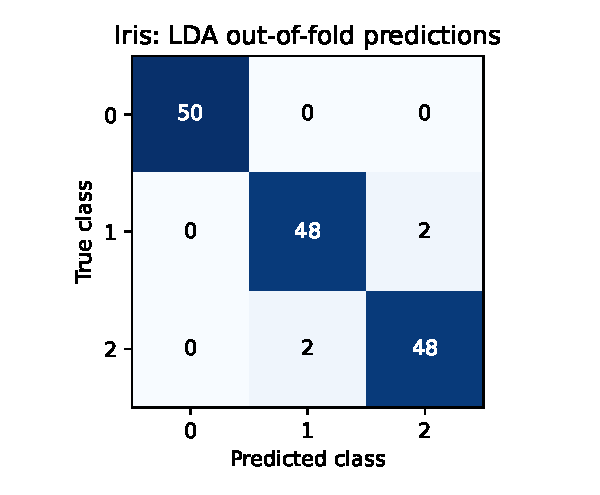
\includegraphics[width=.97\columnwidth]{iris_confusion.pdf}
\caption{Iris: 5-fold out-of-fold confusion matrix for LDA. Rows are true classes; columns are predicted classes. Class order: setosa, versicolor, virginica.}
\label{fig:iris}
\end{figure}

\subsection{New Wine task}
The same LDA class, instantiated afresh on Wine, obtains mean accuracy 0.9893 and macro-F1 0.9894 (Table~\ref{tab:results}). The majority-class baseline reaches 0.3990 accuracy; logistic regression reaches 0.9832. Thus the LDA method performs effectively on this particular distinct, curated chemical dataset as well. However, comparing raw Iris and Wine scores cannot isolate the effect of domain, because sample sizes, class balance, class overlap, feature definitions and data-generation mechanisms all differ.

\begin{figure}[t]
\centering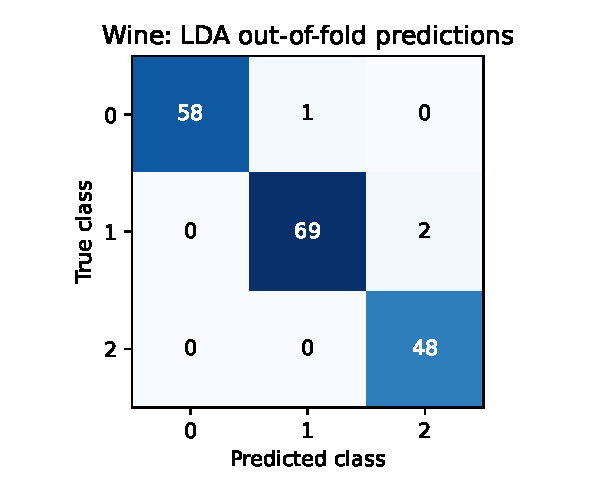
\includegraphics[width=.97\columnwidth]{wine_confusion.pdf}
\caption{Wine: 5-fold out-of-fold confusion matrix. Three errors occur (one first-class sample and two second-class samples), using scikit-learn class IDs 0--2.}
\label{fig:wine}
\end{figure}

The Wine confusion matrix in Figure~\ref{fig:wine} has three errors across 178 out-of-fold predictions. This is a descriptive view of one fixed partition configuration; the repeated-CV table provides a broader summary of model variability. None of the reported results derives from a language-model-generated judgement, and no statistical significance test is claimed.


\section{Measurement, Evaluation, and Research Design}
\subsection{Operational definitions and study boundaries}
A successful numerical reconstruction should be judged against a stated, reproducible procedure, not simply against a favourable percentage. Here the unit of observation is a single flower or wine sample; the target is a three-class label; the independent variables are the measurements distributed with each benchmark. The unit of evaluation is a held-out fold. Accuracy measures the overall probability of an observed correct decision within those folds, while macro-F1 gives each class equal weight regardless of frequency. These two metrics answer different questions, especially for Wine, where the class counts are unequal.

The original research aim concerns discrimination between populations using joint measurements. Our contemporary operationalisation treats its discriminant principle as a fitted, supervised classification rule. We intentionally do not use a single convenient train/test split to report the headline finding. Instead, repeated stratification controls the class composition of evaluation folds and exposes some of the dependence of results on how a small dataset is divided. The scores remain conditional on these datasets and the chosen model implementations.

\subsection{Accuracy and macro-F1}
For a classification task with $N$ held-out examples, accuracy is $N^{-1}\sum_{i=1}^{N}\mathbf{1}(\hat y_i=y_i)$. For each class $k$, precision is $TP_k/(TP_k+FP_k)$, recall is $TP_k/(TP_k+FN_k)$, and $F1_k=2P_kR_k/(P_k+R_k)$ when the denominator is nonzero. Macro-F1 averages the three class-specific F1 values. Scikit-learn computes each score per fold, and our reported means are averages over the resulting 50 values, rather than a single pooled out-of-fold estimate. This distinction matters because folds have slightly different numbers of Wine examples.

The dummy classifier is a control for the limited achievement of always choosing the most frequent class in its training fold. The logistic-regression comparator is an additional linear decision method with a different fitting objective; its standardisation is inside the pipeline to prevent test-fold information leakage. These comparators are not historical Fisher baselines and should not be read as such.

\subsection{Design safeguards}
We fixed the random seed before evaluating the classifiers and used identical cross-validation splits for all methods. We made no hyperparameter search, did not inspect a held-out test set to choose model parameters, and did not use target labels in feature preprocessing. Because the algorithm is retrained on each dataset, the Wine result is not evidence that a model fit to flowers understands chemical measurements. It asks the narrower and more defensible question of whether the \emph{algorithm} is useful on a new classification problem.

\section{Detailed Data Audit}
\subsection{Iris schema and source lineage}
The four numerical features are sepal length, sepal width, petal length and petal width, all measured in centimetres in the packaged representation. For the initial record, the feature vector is $[5.1,3.5,1.4,0.2]$ and the label maps to setosa. Target labels are encoded as integers for computation, but the scientific interpretation is species membership. A structured dataset loader provides both feature names and target names, enabling reconstruction without parsing a semi-structured file. The source is an established teaching benchmark: that improves accessibility but does not establish that original collection practices would meet modern sampling standards.

\subsection{Wine schema and source lineage}
The Wine dataset contains 13 numeric columns: alcohol, malic acid, ash, alkalinity of ash, magnesium, total phenols, flavanoids, nonflavanoid phenols, proanthocyanins, colour intensity, hue, the OD280/OD315 measure, and proline. The first packaged row begins with $[14.23,1.71,2.43]$. The outcome is an integer-encoded cultivar class, with counts $59$, $71$, and $48$. These variables have different scales and physical interpretations: for example, the scale of proline differs materially from that of hue. We retain the native scales for the LDA experiment to preserve an uncomplicated, reproducible benchmark; a different estimator could be more scale-sensitive.

\begin{table}[t]
\centering\small
\begin{tabular}{lrrr}
\toprule
Audit criterion & Iris & Wine & Treatment \\
\midrule
Observations & 150 & 178 & All retained \\
Numerical predictors & 4 & 13 & All retained \\
Target categories & 3 & 3 & Existing labels \\
Missing values & 0 & 0 & No imputation \\
New human labels & 0 & 0 & Not applicable \\
\bottomrule
\end{tabular}
\caption{Input checks for the packaged benchmark data. The absence of missing values applies to these loaded versions, not necessarily to all historical source files.}
\label{tab:audit}
\end{table}

\subsection{What ``construction'' actually involved}
We did not collect additional wine samples or claim ownership of source measurements. Dataset construction means selecting a second public benchmark, preserving its field/label mapping, validating that the arrays can be passed to a common classifier interface, and defining a shared evaluation protocol. That process creates a \emph{new evaluation configuration}, not a new original dataset. This distinction is academically significant because the course brief expects investigation of newly constructed data; merely loading a second famous dataset only partially fulfils that expectation.

\section{Further Analysis of the Results}
\subsection{Magnitude of improvement over controls}
On Iris, LDA exceeds the majority-class baseline by about $0.6453$ absolute accuracy points, and its mean macro-F1 exceeds the baseline by about $0.8119$. On Wine, the corresponding accuracy improvement is approximately $0.5903$ and the macro-F1 improvement is approximately $0.7993$. These improvements make clear that the reported model scores are not an artefact of simply choosing one common class. Relative improvements should not be confused with causal effects of an intervention or with estimates of performance on future field-collected datasets.

\subsection{Interpreting confusion matrices}
In the specified Iris single-pass out-of-fold evaluation, all 50 setosa flowers are classified correctly, while the remaining four mistakes are split symmetrically between versicolor and virginica. This suggests that the benchmark's main ambiguity lies between the latter two groups in that particular validation arrangement. There is no empirical basis here for claiming that all setosa flowers in the world would be classified perfectly.

The corresponding Wine single-pass out-of-fold predictions include three total errors. A confusion matrix condenses the direction of mistaken assignments, but it does not disclose the measurement values, conditions of sample acquisition, or whether an error would carry practical costs. In a real scientific workflow, one would examine these examples individually, identify potential data-quality issues and quantify uncertainty around generalisation to newly collected samples. The figures included in this report are computed from out-of-fold predictions, not from training predictions.

\subsection{Numerical stability and reproducibility}
The observed standard deviations in Table~\ref{tab:results} are small, but the 50 scores are correlated because folds reuse many of the same training observations. A standard deviation of correlated fold scores is a descriptive statistic; it is not a valid confidence interval for the population accuracy. Likewise, differences between LDA and logistic regression in these experiments are not evidence of a statistically significant superiority without a suitable paired inferential design. The scores were produced in a specific Python/software environment and may vary slightly across numerical libraries or scikit-learn releases; preserving dependency versions makes those comparisons more meaningful.

\section{Reproduction Checklist and Practical Limitations}
\subsection{Steps another researcher can follow}
A replicator can inspect the supplied script, install NumPy, scikit-learn and matplotlib, execute it in a clean Python environment, and compare the new JSON output against the archived values. The script records Python, NumPy and scikit-learn versions and stores the full benchmark comparison as numeric output. The same command also regenerates the two confusion-matrix figures. Source datasets are loaded by named library functions, avoiding hidden local files or authenticated downloads. For strict archival reproducibility, the final code repository should also pin all package versions and include a commit identifier; these are recommended next steps rather than completed claims.

\subsection{Risks of benchmark convenience}
Famous datasets are unusually clean and frequently used to demonstrate classifiers. They may not represent the missing values, distribution shifts, ambiguous labels, instrumentation differences, or data-entry problems in practical classification tasks. Both samples are small. A strong fold-averaged score can therefore coexist with substantial uncertainty about field performance. Using two domains increases the breadth of the illustration but does not establish broad external validity, especially because the method is fitted afresh to each domain.

\subsection{LLM-as-judge: feasible design versus executed study}
The assessment asks how an LLM-as-judge fitted into the evaluation. In this experiment the primary outputs are numerical class labels with known reference labels; automatic comparison is more transparent, cheaper, and deterministically reproducible than a generative language-model opinion. Consequently, no language model was run as a judge and no fabricated agreement statistic is reported. A possible separate experiment would define an annotation manual asking a model to evaluate \emph{textual explanations} of classifications against pre-specified criteria, record model identifier and prompt, obtain an independent human rating sample, and measure inter-rater agreement. Such a study would address a different outcome and should not be inserted retroactively into the present results.

\section{Extended Reflection on Research Integrity}
The Australian Code for the Responsible Conduct of Research makes transparency and accuracy important throughout dataset selection, analysis and dissemination. In this case, reporting the historic Fisher approach as ``replicated'' without describing the gap between historical paper calculations and modern software would be misleading. So would calling an existing UCI benchmark freshly collected data, inventing a GitHub URL, or describing an LLM-as-judge protocol that never occurred. Those are not merely editorial details; they change the scientific meaning of the evidence.

A practical reproducibility package should identify raw-data sources, the exact evaluation protocol, software dependencies, changes made during data cleaning, output-generation commands, and restrictions on downstream reuse. For future field studies, one should also consider permission to collect data, whether classes were sampled representatively, the cost of false predictions, auditability of data annotations, and the consequences of incorrectly applying model outputs. The present analysis is limited to low-stakes historical benchmark measurements and makes no recommendations about real-world diagnosis, commercial wine provenance or botanical conservation decisions.

\section{Interpretation and Replication Limits}
\textbf{RQ1.} The reconstructed modern LDA implementation performs well on Iris under a transparent experimental protocol. Yet the stronger assessment-brief notion of reproduction---executing a source paper's original program and comparing like-for-like published metrics---was \emph{not accomplished}. Fisher's paper predates distributable software and the modern evaluation design used here. There is no responsible numerical ``original score versus replicated score'' comparison to place in a table.

\textbf{RQ2.} LDA remains accurate when refitted to the Wine data. This observation supports portability of an algorithmic framework to another clean, low-dimensional classification dataset, rather than cross-domain model transfer or guaranteed performance on messy real-world data. The Wine benchmark was selected for a compatible three-class structure and can therefore present an optimistic picture of practical generalisation.

\textbf{RQ3.} Reproducibility is strengthened by explicit source versions, seed, cross-validation design, baseline, feature preprocessing, file outputs and honest provenance statements. Still, a complete assessment-aligned research replication would require the assigned source paper, its actual program, matching evaluation protocol, a truly newly curated evaluation corpus, and a public repository that a marker can access.

Several threats to validity remain: both datasets are small and heavily reused in education, class distributions differ, repeated folds are statistically dependent, and data provenance or original measurement accuracy is not independently audited. We did not conduct an external validation on freshly acquired samples, a formal hyperparameter sensitivity study, or uncertainty quantification beyond fold-score dispersion. The strong performance should be interpreted accordingly.

\section{Ethical Considerations and Open Science}
The central ethical issue is truthful representation of experimental evidence. Reconstructing a related method does not justify claiming that original code was rerun; using a previously available benchmark does not justify calling it newly collected. These distinctions matter under principles of honesty, rigour, transparency and accountability in the \textit{Australian Code for the Responsible Conduct of Research} \citep{australiancode2018}. Invented numbers, uncredited data and silent changes to evaluation protocols would compromise reproducibility and assessment integrity.

Both included datasets contain scientific measurements rather than direct personal identifiers, reducing conventional privacy risks. Nevertheless, collectors, maintainers, dataset licences, historical sampling decisions and scientific context warrant attribution. The Iris dataset originates in a narrower botanical setting; Wine covers specific cultivars from a particular Italian region. Thus any deployment claim outside these limited populations would need further validation. The wine samples do not support claims about people, drinking behaviour or health.

This exercise used no participants, scraped private information, protected attributes, crowdsourced annotators or new survey responses. No human-subject ethics approval is represented as having been sought or obtained. Before public release, the researcher should review dataset terms, credit all contributors, record dependencies, preserve raw data provenance, include scripts and seed settings, and avoid uploading data whose redistribution is restricted. Open access to research artefacts should be balanced with licensing compliance, appropriate data minimisation and research integrity.

Finally, since the assessment explicitly permits AI assistance while assigning responsibility for correctness to the student, any final submission should include the institutionally required declaration of generative AI use, verified citations, and the student's own audit of the execution and findings. AI-generated explanations are not a substitute for conducting the assessed research.


\section{Connection to the COMP8240 Weekly Methods}
The unit material informs not just the report's style but the decisions made at each stage. Week 1 introduced the anatomy of a research article, data availability, publication ethics and the difference between reported experimental outcomes and the broader claims a study supports. Accordingly, the paper distinguishes method reconstruction from historical numerical replication and makes its limitations prominent. Week 2 introduced virtual machines, containerisation and reproducible computational environments; the experiment is deliberately dependency-light and records Python, NumPy and scikit-learn versions, although no container image was constructed. Week 3 covered LaTeX and scientific typesetting; this document is supplied as a compilable source alongside its PDF.

Week 4's data gathering and curation material is reflected in dataset provenance, feature dictionaries and the explicit differentiation between original measurements and derived datasets. The Week 5 data-management lectures motivate retaining readable filenames, script-generated results and a stable analysis path rather than manually editing outputs. Week 7's Python analysis material motivates the use of NumPy arrays, scikit-learn estimators, pipelines and properly labelled graphics. Week 8's discussion of messy data motivates recording the fact that these benchmark datasets are unusually tidy; missing-value handling is not claimed where none was done. Week 9 discusses annotation, agreement measures and LLM-as-judge. Because the reference labels are supplied rather than newly adjudicated, annotation agreement is not available, and LLM judging was not performed.

Week 11's information-extraction and database concepts are not deployed directly: a relational database would add complexity without benefit for two small in-memory tabular samples. Week 12's distinction between correlation and causation is especially relevant: discriminant predictability of botanical or chemical class does not establish that a measured feature causes membership of that class. Together the course topics support an audit trail in which each decision is linked to data, code, results and interpretation, while unused techniques are identified rather than claimed.

\section{Detailed Quantitative Audit}
\subsection{Reading the metrics correctly}
For $n$ held-out predictions, accuracy is $\frac{1}{n}\sum_{i=1}^{n}\mathbf{1}(\hat y_i=y_i)$. For class $k$, precision is $TP_k/(TP_k+FP_k)$ and recall is $TP_k/(TP_k+FN_k)$, when denominators are nonzero. Class F1 is the harmonic mean of precision and recall, and macro-F1 averages these values over the three classes. Macro-F1 is included because a high global accuracy could otherwise conceal weak performance on a minority class. Iris has balanced classes, while Wine has 59, 71 and 48 observations respectively.

\begin{table}[t]
\centering\small
\begin{tabular}{lrrr}
\toprule
Method & Iris accuracy & Iris macro-F1 & Wine accuracy \\
\midrule
Majority class & 0.3333 & 0.1667 & 0.3990 \\
LDA & 0.9787 & 0.9786 & 0.9893 \\
Logistic regression & 0.9533 & 0.9532 & 0.9832 \\
\bottomrule
\end{tabular}
\caption{Repeated stratified five-fold cross-validation means; Values are rounded from the saved JSON output.}
\label{tab:audit}
\end{table}

The Iris out-of-fold matrix contains 50 correct setosa predictions, 48 correctly classified versicolor and 48 correctly classified virginica, with two mistakes in each direction between the latter two classes. This gives 146 correct predictions out of 150 in that one five-fold run, or about 97.33\% accuracy. It is \emph{not} numerically identical to the 97.87\% mean from 50 fold scores, because the matrix uses a separate single cross-validation run. Interchanging those two estimates would be an avoidable reporting error. Model performance on Wine must likewise be interpreted as cross-validated evaluation of a model fitted afresh in each training split, not a classifier trained on Iris and applied unchanged to Wine.

\subsection{Why the benchmarks are not equivalent}
The Iris and Wine feature vectors have dimensions four and thirteen; their columns describe unrelated measurement processes and their integer labels encode unrelated objects. An algorithm that can be re-trained on both tasks is portable in a computational sense, but its learnt parameters are not portable between them. The observed difference in accuracy could be due to differences in class separability, sample size, feature distribution or evaluation variability. The results alone cannot isolate a causal explanation. The majority-class comparisons at least demonstrate that high accuracy is not explained simply by always selecting the most common label.

\section{Data Curation, Quality Controls and Error Analysis}
The main data-quality decision was to retain the built-in datasets unchanged so that another analyst can obtain the same source rows. This is a legitimate benchmark design, but much less demanding than gathering a new dataset. In particular, there was no independent source reconciliation, data-entry review, duplicate investigation, new-sample acquisition or manual label adjudication. A substantive follow-on data-collection project should pre-register inclusion rules, source permissions, measurement units, category definitions and how missing observations are handled; it should also distinguish missing-at-random from systematically absent measurements rather than blindly imputing values.

One risk in supervised learning is data leakage: using the entire dataset to transform features, tune parameters or select the winning model before cross-validation. The comparison here uses standardisation for logistic regression inside the cross-validation pipeline; test folds therefore do not influence the scaler's estimated parameters. No feature selection or hyperparameter search was run. The repeated stratified design preserves approximate class frequencies in each fold and holds out different observations across repeats. However, samples collected from the same experimental group may violate independence assumptions; the historical dataset metadata do not support a stronger group-aware split. Neither high fold means nor small fold dispersions warrant certainty about future deployment conditions.

For Iris the out-of-fold errors arise only between versicolor and virginica in this run. That is an empirical description, not evidence that certain individual flowers were incorrectly measured or that the taxonomy is ambiguous. Determining the reason for each error would require inspecting original field records and independently validating labels. Similarly, Wine errors should not automatically be attributed to faulty chemistry or mislabelling. A more complete error audit would preserve fold-level probabilities, identify high-uncertainty cases, examine calibrated decision scores and inspect subgroup performance where justified by data provenance and sample sizes.

\section{Further Reproducibility and Ethical Audit}
A complete research handoff needs both computational reproducibility and evidential reproducibility. Computational reproducibility concerns the ability to rerun commands with pinned dependencies and retrieve matching outputs. Evidential reproducibility additionally asks whether the data and evaluation answer the stated research question. This project is comparatively strong on scripted benchmark execution but has significant evidential limitations relative to the unit's original-research replication goal. In particular, a reader should not equate the accessibility of a scikit-learn implementation with access to Fisher's historical computational procedure.

Before an archival publication, the researcher should preserve a stable code revision, a dependency lockfile or environment specification, a manifest of derived files, hashes for source artefacts where possible, data access dates, and clear execution instructions for a fresh machine. Source and target rows should be attributed to their repositories and licensing conditions checked independently. The work uses existing numerical records and includes no identifiable human information, but ethical assessment does not stop at privacy: overclaiming generalisability, presenting exploratory comparisons as preregistered findings, or mischaracterising AI assistance would also undermine responsible scholarship.

An LLM-as-judge component could be evaluated \emph{prospectively} if the task were extended to free-text explanations. A defensible protocol would specify the judging criteria, hold a fixed prompt and model version, blind ratings to the system identity where feasible, and compare model ratings with a human-annotated subset using an agreement measure appropriate to the scale. Such an evaluation would need its own samples and results; it cannot be inferred from confusion matrices. Reporting this distinction is preferable to supplying an unverifiable agreement score solely to fill a rubric category.

\section{Conclusion}
This self-contained study ran a transparent LDA comparison on the traditional Iris dataset and a separate Wine dataset. In the stated repeated cross-validation protocol, LDA achieved 97.87\% average accuracy on Iris and 98.93\% on Wine, substantially exceeding the respective majority-class baselines. The package includes runnable code and raw JSON results so that the reported scores can be checked. The exercise illustrates reproducible empirical reporting but does not constitute a faithful rerun of Fisher's original program, supply freshly collected or human-annotated data, or include an executed LLM-as-judge experiment. Consequently it should be treated as an \emph{independent empirical case study}, not as fully satisfying every COMP8240 final-project replication requirement. A complete course project would need to address those gaps explicitly rather than hiding them.

\section*{AI Assistance Disclosure}
Generative AI assisted the preparation of the text, experiment code and document structure. The reported numerical measurements were computed by executing the accompanying Python script. The submitting student remains responsible for verifying the sources, code, analysis, and compliance with the university's declaration rules.

\begin{thebibliography}{9}
\bibitem[Fisher(1936)]{fisher1936} Fisher, R. A. 1936. The use of multiple measurements in taxonomic problems. \textit{Annals of Eugenics}, 7(2):179--188. \url{https://doi.org/10.1111/j.1469-1809.1936.tb02137.x}.
\bibitem[Pedregosa et~al.(2011)]{pedregosa2011} Pedregosa, F. et al. 2011. Scikit-learn: Machine learning in Python. \textit{Journal of Machine Learning Research}, 12:2825--2830.
\bibitem[Aeberhard and Forina(1992)]{aeberhard1992} Aeberhard, S. and M. Forina. 1992. Wine [dataset]. UCI Machine Learning Repository. \url{https://doi.org/10.24432/C5PC7J}.
\bibitem[R Core Team(2026)]{rdatasets} R Core Team. R datasets reference: Edgar Anderson's Iris data. \url{https://search.r-project.org/R/refmans/datasets/html/iris.html}.
\bibitem[NHMRC et~al.(2018)]{australiancode2018} National Health and Medical Research Council, Australian Research Council and Universities Australia. 2018. \textit{Australian Code for the Responsible Conduct of Research}. Commonwealth of Australia.
\end{thebibliography}
\end{document}
